% benchmarks.tex — \input'd from experiments/experiments.tex
%
% Merges content from the former benchmark.tex and hk2017-optimization.tex.
%
% Sources: experiments/data/polytopes.jsonl (HK2017 timing),
%   experiments/data/pentagon_sweep.jsonl, polygon_grid.jsonl,
%   random_products.jsonl (billiard timing).

\subsection{Benchmarks and Algorithm Selection}
\label{sec:benchmark}

The two capacity algorithms have fundamentally different computational
profiles: HK2017 is exponential in the facet count, while the billiard
algorithm is polynomial but restricted to Lagrangian products. We benchmark
both to establish practical limits and guide algorithm selection in subsequent
experiments.

\subsubsection*{HK2017 implementation optimization}

Before benchmarking, we optimized the HK2017 implementation without changing
the underlying algorithm:

\begin{enumerate}
  \item \textbf{LU fast path.} The KKT solver tries full-pivoting LU
    decomposition before falling back to SVD. Since rank deficiency is rare,
    this avoids the more expensive SVD in $>$95\% of iterations. Speedup:
    3--5$\times$.

  \item \textbf{Lazy permutation generation.} In-place callback via Heap's
    algorithm replaces eager collection of all $(m{-}1)!$ cyclic permutations.
    For $m = 10$, this eliminates 362{,}880 vector allocations. Speedup:
    1.2--2.2$\times$.
\end{enumerate}

Combined wall-clock improvement: 4.6$\times$ on the HK-O pentagon ($F = 10$),
5--6$\times$ on random polytopes at $F = 10$. Peak heap memory dropped from
573\,KB to 17\,KB.

\subsubsection*{HK2017 timing profile}

Table~\ref{tab:benchmark-stats} shows timing statistics for \texttt{ehz\_capacity\_pruned}
on the main polytope dataset (330 random polytopes, $F = 5, \ldots, 12$).

\begin{table}[h]
\centering
\begin{tabular}{rrrrrr}
\toprule
$F$ & $N$ & Median (ms) & Mean (ms) & Min (ms) & Max (ms) \\
\midrule
 5 & 50 &       0.3 &       0.3 &      0.2 &       0.7 \\
 6 & 50 &       1.1 &       1.1 &      0.5 &       2.1 \\
 7 & 50 &       3.3 &       3.4 &      1.7 &       6.1 \\
 8 & 50 &      13.3 &      12.8 &      5.2 &      24.5 \\
 9 & 50 &      58.6 &      61.6 &     21.4 &     141.5 \\
10 & 50 &     273.7 &     303.6 &    104.5 &     636.5 \\
11 & 20 &   1{,}606 &   1{,}804 &    671.0 &   3{,}718 \\
12 & 10 &   9{,}118 &   9{,}260 &   4{,}829 &  13{,}189 \\
\bottomrule
\end{tabular}
\caption{HK2017 computation time for random 4-polytopes by facet count.
  All times measured after LU fast path and lazy permutation optimizations.}
\label{tab:benchmark-stats}
\end{table}

A log-linear regression on the median times yields the exponential model
\[
  T_{\mathrm{HK2017}}(F) \;=\; 1.5 \times 10^{-7} \cdot 4.32^F \quad\text{seconds}
  \qquad (R^2 = 0.994).
\]
The growth rate of~${\sim}4\text{--}5\times$ per facet reflects the combinatorial
explosion: the number of cyclic permutations of a facet subset grows
super-exponentially with~$F$, and adjacency pruning removes a roughly
constant fraction at each level.

\subsubsection*{Billiard timing profile}

On Lagrangian products, the billiard algorithm is dramatically faster. The
algorithm enumerates only 2-bounce and 3-bounce orbit patterns, giving
polynomial cost in the number of facets.

On the \textsc{PentagonSweep} ($F = 10$, 361 points), the billiard algorithm
computes each capacity in ${\sim}173$\,ms (median), compared to
${\sim}477$\,ms for HK2017 --- a speedup of ${\sim}3\times$.
The billiard's advantage grows with facet count because
HK2017's cost is exponential while billiard's is polynomial.

\subsubsection*{Algorithm selection}

\begin{itemize}
  \item \textbf{Lagrangian products}: Always use billiard (polynomial cost,
    cross-validated against HK2017 in Section~\ref{sec:correctness}).
  \item \textbf{General polytopes}: Use HK2017 pruned (the only general
    algorithm). Practical limit: $F \le 12$ for routine datasets, $F \le 14$
    for one-off computations.
  \item \textbf{Debug testing}: Use HK2017 unpruned on $F \le 7$ to exercise
    all code paths with internal assertions enabled. Infeasible for larger
    polytopes due to exponential cost without pruning.
\end{itemize}

Figure~\ref{fig:benchmark-timing} shows the timing data and fitted model
for HK2017.

\begin{figure}[h]
\centering
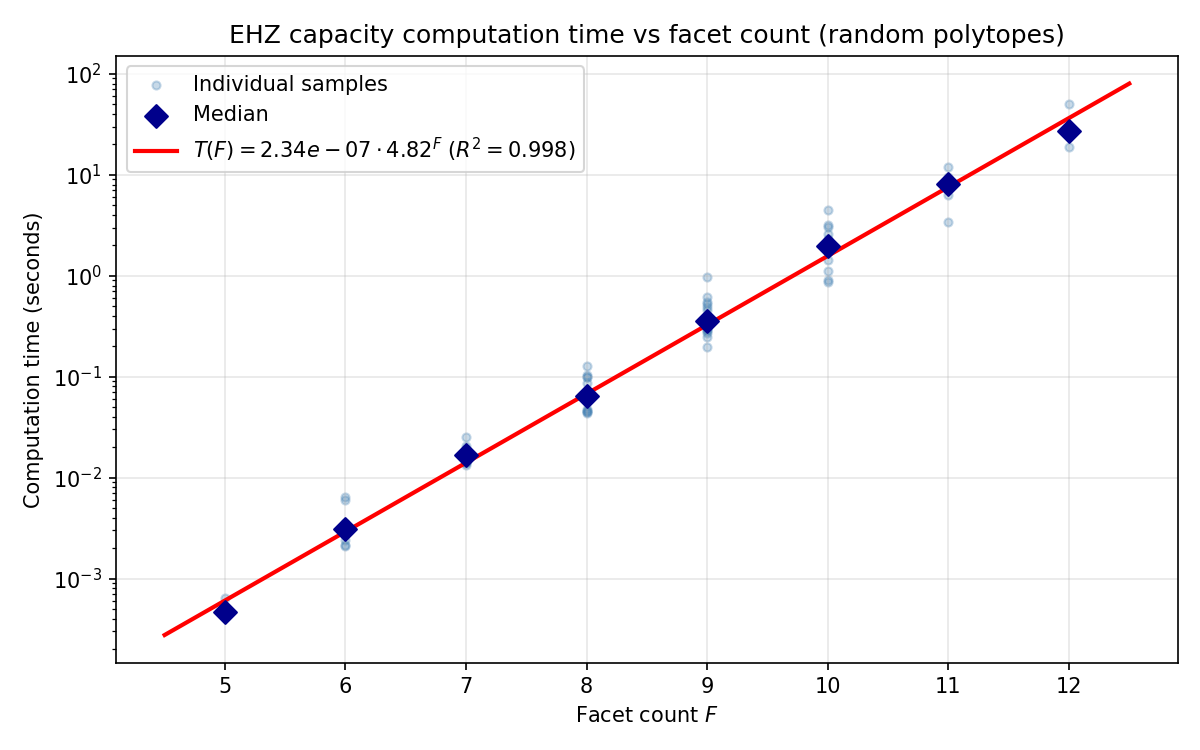
\includegraphics[width=0.75\textwidth]{../experiments/figures/benchmark_timing.png}
\caption{EHZ capacity computation time vs facet count for random polytopes
  (HK2017 pruned). Diamonds: median per facet count. Red line: fitted
  exponential model $T(F) = 1.5 \times 10^{-7} \cdot 4.32^F$.}
\label{fig:benchmark-timing}
\end{figure}
